\chapter{Shared Memory Parallelism} 
\label{chap:shared} 

Shared-memory programming is considered by many in the parallel
processing community as being the clearest of the various parallel
paradigms available.

Note:  To get the most of this section---which is used frequently in the
rest of this book---you may wish to read the material on array storage
in the appendix of this book, Section \ref{arraystorage}.

\section{What Is Shared?}

The term \textbf{shared memory} means that the processors all share a
common address space. Say this is occurring at the hardware level, and
we are using Intel Pentium CPUs.  Suppose processor P3 issues the
instruction

\begin{Verbatim}[fontsize=\relsize{-2}]
movl 200, %ebx
\end{Verbatim}

which reads memory location 200 and places the result in the EAX
register in the CPU.  If processor P4 does the same, they both will be
referring to the same physical memory cell. (Note, however, that each
CPU has a separate register set, so each will have its own independent
EAX.) In non-shared-memory machines, each processor has its own private
memory, and each one will then have its own location 200, completely
independent of the locations 200 at the other processors' memories.

Say a program contains a global variable {\bf X} and a local variable
{\bf Y} on share-memory hardware (and we use shared-memory software). If
for example the compiler assigns location 200 to the variable {\bf X},
i.e.  \verb0&X = 2000, then the point is that all of the processors will
have that variable in common, because any processor which issues a
memory operation on location 200 will access the same physical memory
cell.

On the other hand, each processor will have its own separate run-time
stack.  All of the stacks are in shared memory, but they will be
accessed separately, since each CPU has a different value in its SP
(Stack Pointer) register.  Thus each processor will have its own
independent copy of the local variable {\bf Y}.

To make the meaning of ``shared memory'' more concrete, suppose we have
a bus-based system, with all the processors and memory attached to the
bus. Let us compare the above variables {\bf X} and {\bf Y} here.
Suppose again that the compiler assigns {\bf X} to memory location 200.
Then in the machine language code for the program, every reference to
{\bf X} will be there as 200. Every time an instruction that writes to
{\bf X} is executed by a CPU, that CPU will put 200 into its Memory
Address Register (MAR), from which the 200 flows out on the address
lines in the bus, and goes to memory. This will happen in the same way
no matter which CPU it is. Thus the same physical memory location will
end up being accessed, no matter which CPU generated the reference.

By contrast, say the compiler assigns a local variable {\bf Y} to
something like ESP+8, the third item on the stack (on a 32-bit machine),
8 bytes past the word pointed to by the stack pointer, ESP.  The OS will
assign a different ESP value to each thread, so the stacks of the
various threads will be separate.  Each CPU has its own ESP register,
containing the location of the stack for whatever thread that CPU is
currently running.  So, the value of {\bf Y} will be different for each
thread.

\section{Memory Modules}
\label{banks}

Parallel execution of a program requires, to a large extent, parallel
accessing of memory.  To some degree this is handled by having a cache
at each CPU, but it is also facilitated by dividing the memory into
separate {\bf modules} or {\bf banks}.  This way several memory accesses
can be done simultaneously.

In this section, assume for simplicity that our machine has 32-bit
words.  This is still true for many GPUs, in spite of the widespread use
of 64-bit general-purpose machines today, and in any case, the numbers
here can easily be converted to the 64-bit case.  

Note that this means that consecutive words differ in address by 4.
Let's thus define the word-address of a word to be its ordinary address
divided by 4.  Note that this is also its address with the lowest two
bits deleted.

\subsection{Interleaving}
\label{interleaving}

There is a question of how to divide up the memory into banks.
There are two main ways to do this:

\begin{itemize}

\item [(a)]

{\bf High-order interleaving:} Here consecutive words are in the
\underbar{same} bank (except at boundaries). For example, suppose for
simplicity that our memory consists of word-addresses 0 through 1023,
and that there are four banks, M0 through M3.  Then M0 would contain
word-addresses 0-255, M1 would have 256-511, M2 would have 512-767, and
M3 would have 768-1023.

\item [(b)]

{\bf Low-order interleaving:} Here consecutive addresses are in
consecutive banks (except when we get to the right end). In the
example above, if we used low-order interleaving, then word-address 0
would be in M0, 1 would be in M1, 2 would be in M2, 3 would be in M3, 4
would be back in M0, 5 in M1, and so on.

\end{itemize}

Say we have eight banks.  Then under high-order interleaving, the first
three bits of a word-address would be taken to be the bank number, with
the remaining bits being address within bank.  Under low-order
interleaving, the three least significant bits would be used to determine
bank number.

Low-order interleaving has often been used for {\bf vector processors}.
On such a machine, we might have both a regular add instruction, ADD,
and a vector version, VADD.  The latter would add two vectors together,
so it would need to read two vectors from memory.  If low-order
interleaving is used, the elements of these vectors are spread across
the various banks, so fast access is possible.

A more modern use of low-order interleaving, but with the same
motivation as with the vector processors, is in GPUs (Chapter
\ref{chap:cuda}).

High-order interleaving might work well in matrix applications, for
instance, where we can partition the matrix into blocks, and have
different processors work on different blocks.  In image processing
applications, we can have different processors work on different parts
of the image.  Such partitioning almost never works perfectly---e.g.
computation for one part of an image may need information from another
part---but if we are careful we can get good results.

\subsection{Bank Conflicts and Solutions}
\label{bankclash}

Consider an array {\bf x} of 16 million elements, whose sum we wish to
compute, say using 16 threads.  Suppose we have four memory banks, with
low-order interleaving. 

A naive implementation of the summing code might be

\begin{Verbatim}[fontsize=\relsize{-2},numbers=left]
parallel for thr = 0 to 15
   localsum = 0
   for j = 0 to 999999
      localsum += x[thr*1000000+j]
   grandsum += localsumsum
\end{Verbatim}

In other words, thread 0 would sum the first million elements, thread 1
would sum the second million, and so on.  After summing its portion of
the array, a thread would then add its sum to a grand total.  (The
threads {\it could} of course add to {\bf grandsum} directly in each
iteration of the loop, but this would cause too much traffic to memory,
thus causing slowdowns.)

Suppose for simplicity that there is one address per word (it is usually
one address per byte).

Suppose also for simplicity that the threads run in lockstep, so that they
all attempt to access memory at once.  On a multicore/multiprocessor
machine, this may not occur, but it in fact typically {\it will} occur
in a GPU setting.

A problem then arises.  To make matters simple, suppose that {\bf x}
starts at an address that is a multiple of 4, thus in bank 0.  (The
reader should think about how to adjust this to the other three cases.)
On the very first memory access, thread 0 accesses {\bf x[0]} in bank 0,
thread 1 accesses {\bf x[1000000]}, also in bank 0, and so on---and {\it
these will all be in memory bank 0}!  Thus there will be major
conflicts, hence major slowdown.

A better approach might be to have any given thread work on every
sixteenth element of {\bf x}, instead of on contiguous elements.  Thread
0 would work on {\bf x[1000000]}, {\bf x[1000016]}, {\bf
x[10000032},...; thread 1 would handle {\bf x[1000001]}, {\bf
x[1000017]}, {\bf x[10000033},...; and so on:

\begin{Verbatim}[fontsize=\relsize{-2},numbers=left]
parallel for thr = 0 to 15
   localsum = 0
   for j = 0 to 999999
      localsum += x[16*j+thr]
   grandsum += localsumsum
\end{Verbatim}

Here, consecutive threads work on consecutive elements in {\bf
x}.\footnote{Here thread 0 is considered ``consecutive'' to thread 15,
in a wraparound manner.}  That puts them in separate banks, thus no
conflicts, hence speedy performance.

In general, avoiding bank conflicts is an art, but there are a couple
of approaches we can try.

\begin{itemize}

\item We can rewrite our algorithm, e.g. use the second version of the
above code instead of the first.

\item We can add {\bf padding} to the array.  For instance in the first
version of our code above, we could lengthen the array from 16 million
to 16000016, placing padding in words 1000000, 2000001 and so on.  We'd
tweak our array indices in our code accordingly, and eliminate bank
conflicts that way.

\end{itemize}

In the first approach above, the concept of {\bf stride} often arises.
It is defined to be the distance betwwen array elements in consecutive
accesses by a thread.  In our original code to compute {\bf grandsum},
the stride was 1, since each array element accessed by a thread is 1
past the last access by that thread.  In our second version, the stride
was 16.

Strides of greater than 1 often arise in code that deals with
multidimensional arrays.  Say for example we have two-dimensional array
with 16 columns.  In C/C++, which uses row-major order, access of an
entire column will have a stride of 16.  Access down the main diagonal
will have a stride of 17.

Suppose we have b banks, again with low-order interleaving.  You should
experiment a bit to see that an array access with a stride of s will
access s different banks if and only if s and b are relatively prime,
i.e. the greatest common divisor of s and b is 1.  This can be proven
with group theory.

Another strategy, useful for collections of complex objects, is to set
up {\bf structs of arrays} rather than {\bf arrays of structs}.  Say
for instance we are working with data on workers, storing for each
worker his name, salary and number of years with the firm.  We might
naturally write code like this:

\begin{lstlisting}[numbers=left]
struct {
   char name[25];
   float salary;
   float yrs;
} x[100];
\end{lstlisting}

That gives a 100 structs for 100 workers.  Again, this is very natural,
but it may make for poor memory access patterns.  Salary values for the
various workers will no longer be contiguous, for instance, even though
the {\bf struct}s are contiguous.  This could cause excessive cache
misses.

One solution would be to add padding to each {\bf struct}, so that the
salary values are a word apart in memory.  But another approach would be
to replace the above arrays of {\bf struct}s by a {\bf struct} of
arrays:

\begin{lstlisting}[numbers=left]
struct {
   char *name[]100;
   float salary[100];
   float yrs[100];
} 
\end{lstlisting}

\subsection{Example:  Code to Implement Padding}

As discussed above, array padding is used to try to get better parallel
access to memory banks.  The code below is aimed to provide utilities to
assist in this.  Details are explained in the comments.

\begin{lstlisting}[numbers=left]

// routines to initialize, read and write
// padded versions of a matrix of floats;
// the matrix is nominally mxn, but its
// rows will be padded on the right ends,
// so as to enable a stride of s down each
// column; it is assumed that s >= n

// allocate space for the padded matrix,
// initially empty
float *padmalloc(int m, int n, int s) {
   return(malloc(m*s*sizeof(float)));
}

// store the value tostore in the matrix q,
// at row i, column j; m, n and
// s are as in padmalloc() above
void setter(float *q, int m, int n, int s,
      int i, int j, float tostore) {
   *(q + i*s+j) = tostore;
}

// fetch the value in the matrix q,
// at row i, column j; m, n and s are
// as in padmalloc() above
float getter(float *q, int m, int n, int s,
      int i, int j) {
   return *(q + i*s+j);
}
\end{lstlisting}


\section{Interconnection Topologies}

\subsection{SMP Systems}

A Symmetric Multiprocessor (SMP) system has the following structure:

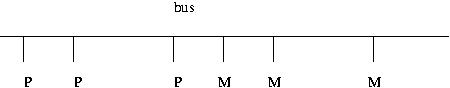
\includegraphics{Images/UMABus.jpg} 

Here and below:

\begin{itemize}

\item The Ps are processors, e.g. off-the-shelf chips such as Pentiums.

\item The Ms are \textbf{memory modules}. These are physically separate
objects, e.g. separate boards of memory chips.  It is typical that there
will be the same number of Ms as Ps. 

\item To make sure only one P uses the bus at a time, standard bus
arbitration signals and/or arbitration devices are used. 

\item There may also be \textbf{coherent caches}, which we will discuss later. 

\end{itemize}

\subsection{NUMA Systems}

In a {\bf Nonuniform Memory Access} (NUMA) architecture, each CPU has a
memory module physically next to it, and these processor/memory (P/M)
pairs are connected by some kind of network.

Here is a simple version:

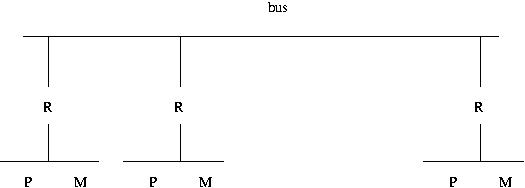
\includegraphics{Images/NUMABus.jpg} 

Each P/M/R set here is called a \textbf{processing element} (PE). Note
that each PE has its own local bus, and is also connected to the global
bus via R, the router.

Suppose for example that P3 needs to access location 200, and suppose
that high-order interleaving is used.  If location 200 is in M3, then
P3's request is satisfied by the local bus.\footnote{This sounds similar
to the concept of a cache. However, it is very different.  A cache
contains a local copy of some data stored elsewhere.  Here it is the
data itself, not a copy, which is being stored locally.} On the other
hand, suppose location 200 is in M8. Then the R3 will notice this, and
put the request on the global bus, where it will be seen by R8, which
will then copy the request to the local bus at PE8, where the request
will be satisfied.  (E.g. if it was a read request, then the response
will go back from M8 to R8 to the global bus to R3 to P3.)

It should be obvious now where NUMA gets its name. P8 will have much
faster access to M8 than P3 will to M8, if none of the buses is
currently in use---and if say the global bus is currently in use, P3
will have to wait a long time to get what it wants from M8.

Today almost all high-end MIMD systems are NUMAs.  One of the attractive
features of NUMA is that by good programming we can exploit the
nonuniformity.  In matrix problems, for example, we can write our
program so that, for example, P8 usually works on those rows of the 
matrix which are stored in M8, P3 usually works on those rows of the
matrix which are stored in M3, etc. In order to do this, we need to make
use of the C language's \& address operator, and have some knowledge of
the memory hardware structure, i.e. the interleaving.

\subsection{NUMA Interconnect Topologies}

The problem with a bus connection, of course, is that there is only one
pathway for communication, and thus only one processor can access memory
at the same time.  If one has more than, say, two dozen processors are
on the bus, the bus becomes saturated, even if traffic-reducing methods
such as adding caches are used. Thus multipathway topologies are used
for all but the smallest systems.  In this section we look at two
alternatives to a bus topology. 

\subsubsection{Crossbar Interconnects}

Consider a shared-memory system with n processors and n memory modules.
Then a crossbar connection would provide \( n^{2} \) pathways. E.g. for n =
8:

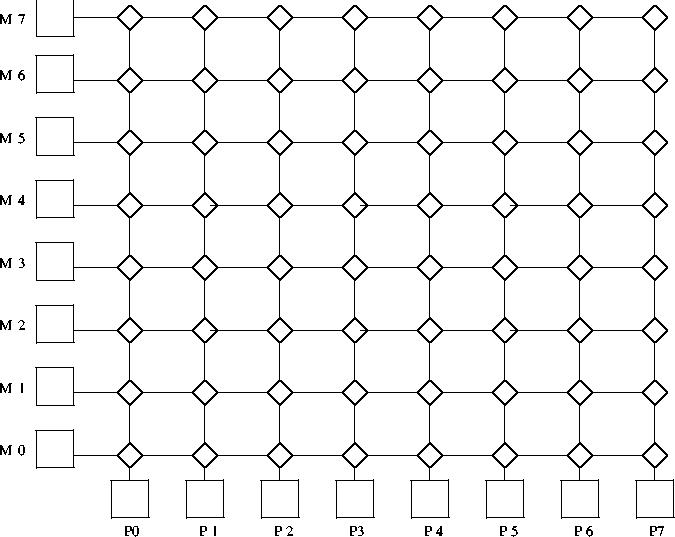
\includegraphics{Images/XBar.jpg} 

Generally serial communication is used from node to node, with a packet
containing information on both source and destination address. E.g. if
P2 wants to read from M5, the source and destination will be 3-bit
strings in the packet, coded as 010 and 101, respectively.  The packet
will also contain bits which specify which word within the module we
wish to access, and bits which specify whether we wish to do a read or a
write.  In the latter case, additional bits are used to specify the
value to be written.

Each diamond-shaped node has two inputs (bottom and right) and two
outputs (left and top), with buffers at the two inputs.  If a buffer
fills, there are two design options: (a) Have the node from which the
input comes block at that output. (b) Have the node from which the input
comes discard the packet, and retry later, possibly outputting some
other packet for now.  If the packets at the heads of the two buffers
both need to go out the same output, the one (say) from the bottom input
will be given priority.

There could also be a return network of the same type, with this one
being memory \( \rightarrow  \) processor, to return the result of the
read requests.\footnote{For safety's sake, i.e. fault tolerance, even
writes are typically acknowledged in multiprocessor systems.}

Another version of this is also possible. It is not shown here, but the
difference would be that at the bottom edge we would have the PEi and at
the left edge the memory modules Mi would be replaced by lines which
wrap back around to PEi, similar to the Omega network shown below.

Crossbar switches are too expensive for large-scale systems, but are
useful in some small systems. The 16-CPU Sun Microsystems Enterprise
10000 system includes a 16x16 crossbar.

\subsubsection{Omega (or Delta) Interconnects}

These are multistage networks similar to crossbars, but with fewer
paths. Here is an example of a NUMA 8x8 system:

\par

\centerline{
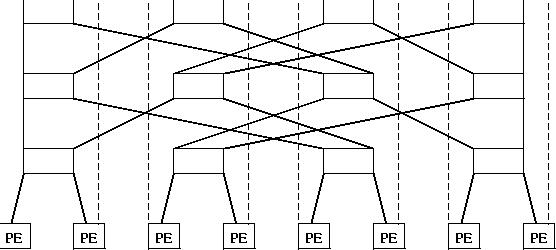
\includegraphics[height=1.0in]{Images/Omega.jpg} 
}

Recall that each PE is a processor/memory pair.  PE3, for instance,
consists of P3 and M3.

Note the fact that at the third stage of the network (top of picture),
the outputs are routed back to the PEs, each of which consists of a
processor and a memory module.\footnote{The picture may be cut off somewhat
at the top and left edges.  The upper-right output of the rectangle in
the top row, leftmost position should connect to the dashed line which
leads down to the second PE from the left.  Similarly, the upper-left
output of that same rectangle is a dashed lined, possibly invisible in
your picture, leading down to the leftmost PE.}

At each network node (the nodes are the three rows of rectangles), the
output routing is done by destination bit. Let's number the stages here
0, 1 and 2, starting from the bottom stage, number the nodes within a
stage 0, 1, 2 and 3 from left to right, number the PEs from 0 to 7, left
to right, and number the bit positions in a destination address 0, 1 and
2, starting from the most significant bit. Then at stage i, bit i of the
destination address is used to determine routing, with a 0 meaning
routing out the left output, and 1 meaning the right one.

Say P2 wishes to read from M5. It sends a read-request packet, including
5 = 101 as its destination address, to the switch in stage 0, node 1.
Since the first bit of 101 is 1, that means that this switch will route
the packet out its right-hand output, sending it to the switch in stage
1, node 3. The latter switch will look at the next bit in 101, a 0, and
thus route the packet out its left output, to the switch in stage 2,
node 2. Finally, that switch will look at the last bit, a 1, and output
out its right-hand output, sending it to PE5, as desired. M5 will
process the read request, and send a packet back to PE2, along the same

Again, if two packets at a node want to go out the same output, one must
get priority (let's say it is the one from the left input).

Here is how the more general case of N = \( 2^{n} \) PEs works. Again
number the rows of switches, and switches within a row, as above. So, \(
S_{ij} \) will denote the switch in the i-th row from the bottom and
j-th column from the left (starting our numbering with 0 in both cases).
Row i will have a total of N input ports \( I_{ik} \) and N output ports
\( O_{ik} \), where k = 0 corresponds to the leftmost of the N in each
case. Then if row i is not the last row (\( i<n-1 \)), \( O_{ik} \) will
be connected to \( I_{jm} \), where j = i+1 and

\begin{equation}
m = (2k + \lfloor (2k)/N \rfloor ) ~ mod ~ N
\end{equation}

If row i is the last row, then \( O_{ik} \) will be connected to, PE k.


\subsection{Comparative Analysis}

In the world of parallel architectures, a key criterion for a proposed
feature is \textbf{scalability}, meaning how well the feature performs
as we go to larger and larger systems. Let n be the system size, either
the number of processors and memory modules, or the number of PEs. Then
we are interested in how fast the latency, bandwidth and cost grow with
n:

\begin{tabular}{|l|r|r|r|}
\hline 
criterion &
 bus &
 Omega&
 crossbar \\
\hline 
latency &
 O(1) &
 $\rm O( \log_2 n)$ &
 O(n) \\
\hline 
bandwidth &
 O(1) &
 O(n) &
 O(n) \\
\hline 
cost &
 O(1) &
 $\rm O(n \log_2 n)$ &
$\rm  O(n^2)$ \\
\hline
\end{tabular}

Let us see where these expressions come from, beginning with a bus: No
matter how large n is, the time to get from, say, a processor to a
memory module will be the same, thus O(1). Similarly, no matter how
large n is, only one communication can occur at a time, thus again
O(1).\footnote{ Note that the `1' in ``O(1)'' does not refer to the fact
that only one communication can occur at a time. If we had, for example,
a two-bus system, the bandwidth would still be O(1), since
multiplicative constants do not matter. What O(1) means, again, is that
as n grows, the bandwidth stays at a multiple of 1, i.e.  stays
constant.  }

Again, we are interested only in ``O( )'' measures, because we are only
interested in growth rates as the system size n grows. For instance, if
the system size doubles, the cost of a crossbar will quadruple; the \(
O(n^{2}) \) cost measure tells us this, with any multiplicative constant
being irrelevant.

For Omega networks, it is clear that \( log_{2}n \) network rows are
needed, hence the latency value given. Also, each row will have n/2
switches, so the number of network nodes will be O(n \( log_{2}n \)).
This figure then gives the cost (in terms of switches, the main expense
here). It also gives the bandwidth, since the maximum number of
simultaneous transmissions will occur when all switches are sending at
once.

Similar considerations hold for the crossbar case.

The crossbar's big advantage is that it is guaranteed that n packets can
be sent simultaneously, providing they are to distinct
destinations.

That is \underbar{not} true for Omega-networks. If for example, PE0
wants to send to PE3, and at the same time PE4 wishes to sent to PE2,
the two packets will clash at the leftmost node of stage 1, where the
packet from PE0 will get priority.

On the other hand, a crossbar is very expensive, and thus is dismissed
out of hand in most modern systems. Note, though, that an equally
troublesom aspect of crossbars is their high latency value; this is a
big drawback when the system is not heavily loaded.

The bottom line is that Omega-networks amount to a compromise between
buses and crossbars, and for this reason have become popular.

\subsection{Why Have Memory in Modules?}

In the shared-memory case, the Ms collectively form the entire
shared address space, but with the addresses being assigned to the Ms in
one of two ways:

\begin{itemize}

\item (a)

High-order interleaving. Here consecutive addresses are in the
\underbar{same} M (except at boundaries). For example, suppose for
simplicity that our memory consists of addresses 0 through 1023, and
that there are four Ms.  Then M0 would contain addresses 0-255, M1 would
have 256-511, M2 would have 512-767, and M3 would have 768-1023.

\item (b)

Low-order interleaving. Here consecutive addresses are in consecutive
M's (except when we get to the right end). In the example above, if we
used low-order interleaving, then address 0 would be in M0, 1 would be
in M1, 2 would be in M2, 3 would be in M3, 4 would be back in M0, 5 in
M1, and so on.

\end{itemize}

The idea is to have several modules busy at once, say in conjunction
with a {\bf split-transaction bus}.  Here, after a processor makes a
memory request, it relinquishes the bus, allowing others to use it while
the memory does the requested work.  Without splitting the memory into
modules, this wouldn't achieve parallelism.  The bus does need extra
lines to identify which processor made the request.

% \subsubsection{Dealing with Latency Problems}
% 
% The hardware and software may also be designed to reduce latency. One
% approach to this is \textbf{latency hiding}, which consists of
% prefetching a word or words from a certain section of memory which is to
% be used soon. It is somewhat similar to the idea of delayed branch in
% RISC processors. Suppose for instance we have code like
% 
% \begin{verbatim}
% LD R4,200
% ADD R5,R2
% ADD R5,R3
% SUB R4,R5
% \end{verbatim}
% 
% (where the Ri are registers).  The hardware design may be such that
% there is a PF (prefetch) instruction, which is \textbf{nonblocking},
% meaning that subsequent instructions can execute while the PF is still
% pending (as long as the subsequent instructions do not depend on the
% result of the PF). Then we could rewrite the above code as
% 
% \begin{verbatim}
% PF R4,200
% ADD R5,R2
% ADD R1,R2
% SUB R4,R5
% \end{verbatim}
% 
% Hopefully the PF will be done by the time we get to the SUB instruction.
% If not, SUB will block for the remaining time, but even then we will
% have saved time.


% \subsubsection{Internode Synchronization on Shared-Memory Hardware}

\section{Synchronization Hardware}

Avoidance of race conditions, e.g. implementation of locks, plays such a
crucial role in shared-memory parallel processing that hardware
assistance is a virtual necessity.  Recall, for instance, that critical
sections can effectively serialize a parallel program.  Thus efficient
implementation is crucial.

\subsection{Test-and-Set Instructions}

Consider a bus-based system. In addition to whatever memory read and
memory write instructions the processor included, there would also be a
TAS instruction.\footnote{This discussion is for a mythical machine, but
any real system works in this manner.}  This instruction would control a
TAS pin on the processor chip, and the pin in turn would be connected to
a TAS line on the bus.

Applied to a location L in memory and a register R, say, TAS does the
following:

\begin{Verbatim}[fontsize=\relsize{-2}]
   copy L to R
   if R is 0 then write 1 to L 
\end{Verbatim}

And most importantly, these operations are done in an \textbf{atomic}
manner; no bus transactions by other processors may occur between the
two steps.

The TAS operation is applied to variables used as locks. Let's say that
1 means locked and 0 unlocked. Then the guarding of a critical section C
by a lock variable L, using a register R, would be done by having the
following code in the program being run:

\begin{Verbatim}[fontsize=\relsize{-2}]
   TRY:  TAS R,L
         JNZ TRY
     C:  ...   ; start of critical section
         ...
         ...   ; end of critical section
         MOV 0,L  ; unlock
\end{Verbatim}

where of course JNZ is a jump-if-nonzero instruction, and we are
assuming that the copying from the Memory Data Register to R results in
the processor N and Z flags (condition codes) being affected.

\subsubsection{LOCK Prefix on Intel Processors}
\label{lockprefix}


On Pentium machines, the LOCK prefix can be used to get atomicity for
certain instructions:  ADD, ADC, AND, BTC, BTR, BTS, CMPXCHG, DEC, INC,
NEG, NOT, OR, SBB, SUB, XOR, XADD.  The bus will be locked for the
duration of the execution of the instruction, thus setting up atomic
operations.  There is a special LOCK line in the control bus for this
purpose.  (Locking thus only applies to these instructions in forms in
which there is an operand in memory.) By the way, XCHG asserts this
LOCK\# bus signal even if the LOCK prefix is not specified.

For example, consider our count-the-2s example on  page
\pageref{count2s}.  If we store {\bf mycount} in a register, say EDX,
then

\begin{lstlisting}
lock add %edx, overallcount
\end{lstlisting}

would replace the code we had earlier,

\begin{lstlisting}
pthread_mutex_lock(&nextbaselock);
overallcount += mylocalcount;
pthread_mutex_unlock(&nextbaselock);
\end{lstlisting}

without locks!

Here is how we could implement a lock if needed.  The lock would be in a
variable named, say, {\bf lockvar}.

\begin{lstlisting}
   movl $lockvar, %ebx
   movl $1, %ecx
top:
   movl $0, %eax
   lock cmpxchg (%ebx), %ecx
   jz top  # else leave the loop and enter the critical section
\end{lstlisting}

The operation CMPXCHG has EAX as an unnamed operand.  The instruction
basically does (here {\bf source} is ECX and {\bf destination} is {\bf
lockvar})

\begin{lstlisting}
if c(EAX) != c(destination)  # sorry, lock is already locked
   c(EAX) <- c(destination)
   ZF <- 0  # the Zero Flag in the EFLAGS register
else
   c(destination) <- c(source)  # lock the lock
   ZF <- 1
\end{lstlisting}

The LOCK prefix locks the bus for the entire duration of the
instruction.  Note that the ADD instruction here involves two memory
transactions---one to read the old value of {\bf overallcount}, and the
second the write the new, incremented value back to {\bf overallcount}.
So, we are locking for a rather long time, potentially compromising
performance when other threads want to access memory, but the benefits
can be huge.

\subsubsection{Locks with More Complex Interconnects}

In crossbar or $\Omega$-network systems, some 2-bit field in the packet
must be devoted to transaction type, say 00 for Read, 01 for Write and
10 for TAS.  In a sytem with 16 CPUs and 16 memory modules, say, the
packet might consist of 4 bits for the CPU number, 4 bits for the memory
module number, 2 bits for the transaction type, and 32 bits for the data
(for a write, this is the data to be written, while for a read, it would
be the requested value, on the trip back from the memory to the CPU).

But note that the atomicity here is best done at the memory, i.e. some
hardware should be added at the memory so that TAS can be done;
otherwise, an entire processor-to-memory path (e.g. the bus in a
bus-based system) would have to be locked up for a fairly long time,
obstructing even the packets which go to other memory modules.

\subsection{May Not Need the Latest}

Note carefully that in many settings it may not be crucial to get the
most up-to-date value of a variable.  For example, a program may have a
data structure showing work to be done.  Some processors occasionally
add work to the queue, and others take work from the queue.  Suppose the
queue is currently empty, and a processor adds a task to the queue, just
as another processor is checking the queue for work.  As will be seen
later, it is possible that even though the first processor has written
to the queue, the new value won't be visible to other processors for
some time.  But the point is that if the second processor does not see
work in the queue (even though the first processor has put it there),
the program will still work correctly, albeit with some performance
loss. 

\subsection{Fetch-and-Add Instructions} 
\label{fanda}

\setlength{\parindent}{0in}

Another form of interprocessor synchronization is a
\textbf{fetch-and-add} (FA) instruction.  The idea of FA is as follows.
For the sake of simplicity, consider code like

\begin{Verbatim}[fontsize=\relsize{-2}]
LOCK(K);
Y = X++;
UNLOCK(K);
\end{Verbatim}

Suppose our architecture's instruction set included an F\&A instruction.
It would add 1 to the specified location in memory, and return the old
value (to {\bf Y}) that had been in that location before being incremented.
And all this would be an atomic operation.

We would then replace the code above by a library call, say,

\begin{Verbatim}[fontsize=\relsize{-2}]
FETCH_AND_ADD(X,1);
\end{Verbatim}

The C code above would compile to, say,

\begin{Verbatim}[fontsize=\relsize{-2}]
F&A X,R,1
\end{Verbatim}

where {\bf R} is the register into which the old (pre-incrementing)
value of {\bf X} would be returned.

There would be hardware adders placed at each memory module. That means
that the whole operation could be done in one round trip to memory.
Without F\&A, we would need two round trips to memory just for the

\begin{Verbatim}[fontsize=\relsize{-2}]
X++;
\end{Verbatim}

(we would load {\bf X} into a register in the CPU, increment the register, and
then write it back to {\bf X} in memory), and then the LOCK() and UNLOCK()
would need trips to memory too.  This could be a huge time savings,
especially for long-latency interconnects.

\section{Cache Issues}
\label{cacheissues}

If you need a review of cache memories or don't have background in that
area at all, read Section \ref{cache} in the appendix of this book
before continuing.

\subsection{Cache Coherency}
\label{cachecoherency}

Consider, for example, a bus-based system. Relying purely on TAS for
interprocessor synchronization would be unthinkable: As each processor
contending for a lock variable spins in the loop shown above, it is
adding tremendously to bus traffic.

An answer is to have caches at each processor.\footnote{The reader may
wish to review the basics of caches.  See for example 
\url{http://heather.cs.ucdavis.edu/~matloff/50/PLN/CompOrganization.pdf}.}
These will store copies of the values of lock variables.  (Of course,
non-lock variables are stored too.  However, the discussion here will
focus on effects on lock variables.) The point is this: Why keep looking
at a lock variable L again and again, using up the bus bandwidth? L may
not change value for a while, so why not keep a copy in the cache,
avoiding use of the bus?

The answer of course is that eventually L \underbar{will} change value,
and this causes some delicate problems. Say for example that processor
P5 wishes to enter a critical section guarded by L, and that processor
P2 is already in there. During the time P2 is in the critical section,
P5 will spin around, always getting the same value for L (1) from C5,
P5's cache. When P2 leaves the critical section, P2 will set L to
0---and now C5's copy of L will be incorrect. This is the \textbf{cache
coherency problem}, inconsistency between caches.

A number of solutions have been devised for this problem. For bus-based
systems, \textbf{snoopy} protocols of various kinds are used, with the
word ``snoopy'' referring to the fact that all the caches monitor
(``snoop on'') the bus, watching for transactions made by
\underbar{other} caches.

The most common protocols are the \textbf{invalidate} and
\textbf{update} types.  This relation between these two is somewhat
analogous to the relation between \textbf{write-back} and
\textbf{write-through} protocols for caches in uniprocessor systems:

\begin{itemize}

\item Under an invalidate protocol, when a processor writes to a
variable in a cache, it first (i.e. before actually doing the write)
tells each other cache to mark as invalid its cache line (if any) which
contains a copy of the variable.\footnote{We will follow commonly-used
terminology here, distinguishing between a {\it cache line} and a {\it
memory block}.  Memory is divided in blocks, some of which have copies
in the cache.  The cells in the cache are called {\it cache lines}.  So,
at any given time, a given cache line is either empty or contains a copy
(valid or not) of some memory block.} Those caches will be updated only
later, the next time their processors need to access this cache line.  

\item For an update protocol, the processor which writes to the variable
tells all other caches to immediately update their cache lines
containing copies of that variable with the new value. 

\end{itemize}

Let's look at an outline of how one implementation (many variations exist)
of an invalidate protocol would operate:

In the scenario outlined above, when P2 leaves the critical section, it
will write the new value 0 to L. Under the invalidate protocol, P2 will
post an invalidation message on the bus. All the other caches will
notice, as they have been monitoring the bus. They then mark their
cached copies of the line containing L as invalid.

Now, the next time P5 executes the TAS instruction---which will be very
soon, since it is in the loop shown above---P5 will find that the copy
of L in C5 is invalid. It will respond to this cache miss by going to
the bus, and requesting P2 to supply the ``real'' (and valid) copy of
the line containing L.

But there's more.  Suppose that all this time P6 had also been executing
the loop shown above, along with P5.  Then P5 and P6 may have to contend
with each other.  Say P6 manages to grab possession of the bus
first.\footnote{Again, remember that ordinary bus arbitration methods
would be used.} P6 then executes the TAS again, which finds L = 0 and
changes L back to 1.  P6 then relinquishes the bus, and enters the
critical section.  Note that in changing L to 1, P6 also sends an
invalidate signal to all the other caches.  So, when P5 tries its
execution of the TAS again, it will have to ask P6 to send a valid copy
of the block.  P6 does so, but L will be 1, so P5 must resume executing
the loop. P5 will then continue to use its valid local copy of L each
time it does the TAS, until P6 leaves the critical section, writes 0 to
L, and causes another cache miss at P5, etc.

At first the update approach seems obviously superior, and actually, if
our shared, cacheable\footnote{ Many modern processors, including
Pentium and MIPS, allow the programmer to mark some blocks as being
noncacheable.} variables were only lock variables, this might be true.

But consider a shared, cacheable vector. Suppose the vector fits into
one block, and that we write to each vector element sequentially. Under
an update policy, we would have to send a new message on the bus/network
for each component, while under an invalidate policy, only one message
(for the first component) would be needed. If during this time the other
processors do not need to access this vector, all those update messages,
and the bus/network bandwidth they use, would be wasted.

Or suppose for example we have code like

\begin{Verbatim}[fontsize=\relsize{-2}]
Sum += X[I];
\end{Verbatim}

in the middle of a \textbf{for} loop. Under an update protocol, we would
have to write the value of Sum back many times, even though the other
processors may only be interested in the final value when the loop ends.
(This would be true, for instance, if the code above were part of a
critical section.)

Thus the invalidate protocol works well for some kinds of code, while
update works better for others.  The CPU designers must try to
anticipate which protocol will work well across a broad mix of
applications.\footnote{Some protocols change between the two modes
dynamically.}

Now, how is cache coherency handled in non-bus shared-memory systems,
say crossbars?  Here the problem is more complex. Think back to the bus
case for a minute: The very feature which was the biggest negative
feature of bus systems---the fact that there was only one path between
components made bandwidth very limited---is a very \underbar{positive}
feature in terms of cache coherency, because it makes
\underbar{broadcast} very easy: Since everyone is attached to that
single pathway, sending a message to all of them costs no more than
sending it to just one---we get the others for free. That's no longer
the case for multipath systems. In such systems, extra copies of the
message must be created for each path, adding to overall traffic.

A solution is to send messages only to ``interested parties.'' In
\textbf{directory-based} protocols, a list is kept of all caches
which currently have valid copies of all blocks. In one common
implementation, for example, while P2 is in the critical section above,
it would be the \textbf{owner} of the block containing L. (Whoever is
the latest node to write to L would be considered its current owner.) It
would maintain a directory of all caches having valid copies of that
block, say C5 and C6 in our story here. As soon as P2 wrote to L, it
would then send either invalidate or update packets (depending on which
type was being used) to C5 and C6 (and \underbar{not} to other caches
which didn't have valid copies).

There would also be a directory at the memory, listing the current
owners of all blocks. Say for example P0 now wishes to ``join the
club,'' i.e. tries to access L, but does not have a copy of that block
in its cache C0.  C0 will thus not be listed in the directory for this
block.  So, now when  it tries to access L and it will get a cache miss.
P0 must now consult the {\bf home} of L, say P14.  The home might be
determined by L's location in main memory according to high-order
interleaving; it is the place where the main-memory version of L
resides.  A table at P14 will inform P0 that P2 is the current owner of
that block. P0 will then send a message to P2 to add C0 to the list of
caches having valid copies of that block.  Similarly, a cache might
``resign'' from the club, due to that cache line being replaced, e.g. in
a LRU setting, when some other cache miss occurs. 

\subsection{Example: the MESI Cache Coherency Protocol}

Many types of cache coherency protocols have been proposed and used,
some of them quite complex. A relatively simple one for snoopy bus
systems which is widely used is MESI, which for example is the protocol
used in the Pentium series.

MESI is an invalidate protocol for bus-based systems.  Its name stands
for the four states a given cache line can be in for a given CPU: 

\begin{itemize}

\item Modified
\item Exclusive
\item Shared
\item Invalid

\end{itemize}

Note that {\it each memory block} has such a state at {\it each cache}.
For instance, block 88 may be in state S at P5's and P12's caches but in
state I at P1's cache.

Here is a summary of the meanings of the states:


\begin{tabular}{|c|c|}
\hline 
state&
 meaning\\
\hline 
M&
 written to more than once; no other copy valid\\
\hline 
E&
 valid; no other cache copy valid; memory copy valid\\
\hline 
S&
 valid; at least one other cache copy valid\\
\hline 
I&
 invalid (block either not in the cache or present but incorrect) \\
\hline 
\end{tabular}

\par{} \vspace{0.3cm}

Following is a summary of MESI state changes.\footnote{See \emph{Pentium
Processor System Architecture}, by D. Anderson and T.  Shanley,
Addison-Wesley, 1995. We have simplified the presentation here, by
eliminating certain programmable options.} When reading it, keep in mind
again that there is a separate state for each cache/memory block combination.

In addition to the terms \textbf{read hit}, \textbf{read miss},
\textbf{write} \textbf{hit}, \textbf{write miss}, which you are already
familiar with, there are also \textbf{read snoop} and \textbf{write
snoop}.  These refer to the case in which our CPU observes on the bus a
block request by another CPU that has attempted a read or write action
but encountered a miss in its own cache; if our cache has a valid copy
of that block, we must provide it to the requesting CPU (and in some
cases to memory).

So, here are various events and their corresponding state changes:

{\bf If our CPU does a read:} 

\begin{tabular}{|c|c|c|}
\hline 
present state&
 event&
 new state\\
\hline 
M&
 read hit&
 M\\
\hline 
E&
 read hit&
 E\\
\hline 
S&
 read hit&
 S\\
\hline 
I&
 read miss; no valid cache copy at any other CPU &
 E\\
\hline 
I&
 read miss; at least one valid cache copy in some other CPU &
 S  \\
\hline 
\end{tabular}

\par{} \vspace{0.3cm}

{\bf If our CPU does a memory write:}

\begin{tabular}{|c|c|c|}
\hline 
present state&
 event&
 new state\\
\hline 
M&
 write hit; do not put invalidate signal on bus; do not update memory&
 M\\
\hline 
E&
 same as M above&
 M\\
\hline 
S&
 write hit; put invalidate signal on bus; update memory&
 E\\
\hline 
I&
 write miss; update memory but do nothing else&
 I  \\
\hline 
\end{tabular}

\par{} \vspace{0.3cm}

{\bf If our CPU does a read or write snoop:}

\begin{tabular}{|c|c|c|}
\hline 
present state&
 event&
 newstate\\
\hline 
M&
 read snoop; write line back to memory, picked up by other CPU&
 S\\
\hline 
M&
 write snoop; write line back to memory, signal other CPU now OK to do its
 write&
 I\\
\hline 
E&
 read snoop; put shared signal on bus; no memory action&
 S\\
\hline 
E&
 write snoop; no memory action&
 I\\
\hline 
S&
 read snoop&
 S\\
\hline 
S&
 write snoop&
 I\\
\hline 
I&
 any snoop&
 I \\
\hline 
\end{tabular}

Note that a write miss does NOT result in the associated block being
brought in from memory.  

Example:  Suppose a given memory block has state M at processor A but
has state I at processor B, and B attempts to write to the block.  B
will see that its copy of the block is invalid, so it notifies the other
CPUs via the bus that it intends to do this write.  CPU A sees this
announcement, tells B to wait, writes its own copy of the block
back to memory, and then tells B to go ahead with its write.  The
latter action means that A's copy of the block is not correct anymore,
so the block now has state I at A.  B's action does not cause loading of
that block from memory to its cache, so the block still has state I at
B.

\par{} \vspace{0.3cm}

\subsection{The Problem of ``False Sharing''}

Consider the C declaration

\begin{Verbatim}[fontsize=\relsize{-2}]
int W,Z;
\end{Verbatim}

Since {\bf W} and {\bf Z} are declared adjacently, most compilers will
assign them contiguous memory addresses.  Thus, unless one of them is at
a memory block boundary, when they are cached they will be stored in the
same cache line.  Suppose the program writes to {\bf Z}, and our system
uses an invalidate protocol.  Then {\bf W} will be considered invalid at
the other processors, even though its values at those processors' caches
are correct.  This is the {\bf false sharing} problem, alluding to the
fact that the two variables are sharing a cache line even though they
are not related.

This can have very adverse impacts on performance.  If for instance our
variable {\bf W} is now written to, then {\bf Z} will suffer unfairly,
as its copy in the cache will be considered invalid even though it is
perfectly valid.  This can lead to a ``ping-pong'' effect, in which
alternate writing to two variables leads to a cyclic pattern of
coherency transactions. 

One possible solution is to add padding, e.g. declaring {\bf W} and {\bf
Z} like this:

\begin{Verbatim}[fontsize=\relsize{-2}]
int W,U[1000],Z;
\end{Verbatim}

to separate {\bf W} and {\bf Z} so that they won't be in the same cache
block.  Of course, we must take block size into account, and check
whether the compiler really has placed the two variables are in widely
separated locations.  To do this, we could for instance run the code

\begin{Verbatim}[fontsize=\relsize{-2}]
printf("%x %x\n,&W,&Z);
\end{Verbatim}

\section{Memory-Access Consistency Policies}
\label{consistency}

Though the word {\it consistency} in the title of this section may seem
to simply be a synonym for {\it coherency} from the last section, and
though there actually is some relation, the issues here are quite
different.  In this case, it is a timing issue:  After one processor
changes the value of a shared variable, when will that value be
visible to the other processors? 

There are various reasons why this is an issue.  For example, many
processors, especially in multiprocessor systems, have {\bf write
buffers}, which save up writes for some time before actually sending
them to memory.  (For the time being, let's suppose there are no
caches.) The goal is to reduce memory access costs.  Sending data to
memory in groups is generally faster than sending one at a time, as the
overhead of, for instance, acquiring the bus is amortized over many
accesses.  Reads following a write may proceed, without waiting for the
write to get to memory, except for reads to the same address.  So in a
multiprocessor system in which the processors use write buffers, there
will often be some delay before a write actually shows up in memory.

A related issue is that operations may occur, or appear to occur, out of
order.  As noted above, a read which follows a write in the program may
execute before the write is sent to memory.  Also, in a multiprocessor
system with multiple paths between processors and memory modules, two
writes might take different paths, one longer than the other, and arrive
``out of order.''  In order to simplify the presentation here, we will
focus on the case in which the problem is due to write buffers, though.

The designer of a multiprocessor system must adopt some {\bf consistency
model} regarding situations like this.  The above discussion shows that
the programmer must be made aware of the model, or risk getting
incorrect results.  Note also that different consistency models will
give different levels of performance.  The ``weaker'' consistency models
make for faster machines but require the programmer to do more work.

The strongest consistency model is Sequential Consistency.  It
essentially requires that memory operations done by one processor
are observed by the other processors to occur in the same order as
executed on the first processor.  Enforcement of this requirement makes
a system slow, and it has been replaced on most systems by weaker
models.

One such model is {\bf release consistency}.  Here the processors' instruction
sets include instructions ACQUIRE and RELEASE.  Execution of an ACQUIRE
instruction at one processor involves telling all other processors to
flush their write buffers.  However, the ACQUIRE won't execute until
pending RELEASEs are done.  Execution of a RELEASE basically means that
you are saying, "I'm done writing for the moment, and wish to allow
other processors to see what I've written."  An ACQUIRE waits for all
pending RELEASEs to complete before it executes.\footnote{There are many
variants of all of this, especially in the software distibuted shared
memory realm, to be discussed later.}  

A related model is {\bf scope consistency}.  Say a variable, say {\bf
Sum}, is written to within a critical section guarded by LOCK and UNLOCK
instructions.  Then under scope consistency any changes made by one
processor to {\bf Sum} within this critical section would then be
visible to another processor when the latter next enters this critical
section.  The point is that memory update is postponed until it is
actually needed.  Also, a barrier operation (again, executed at the
hardware level) forces all pending memory writes to complete.

All modern processors include instructions which implement consistency
operations.  For example, Sun Microsystems' SPARC has a MEMBAR
instruction.  If used with a STORE operand, then all pending writes at
this processor will be sent to memory.  If used with the LOAD operand,
all writes will be made visible to this processor.

Now, how does cache coherency fit into all this?  There are many
different setups, but for example let's consider a design in which there
is a write buffer between each processor and its cache.  As the
processor does more and more writes, the processor saves them up in the
write buffer.  Eventually, some programmer-induced event, e.g. a MEMBAR
instruction,\footnote{We call this ``programmer-induced,'' since the
programmer will include some special operation in her C/C++ code which
will be translated to MEMBAR.} will cause the buffer to be flushed.
Then the writes will be sent to ``memory''---actually meaning that they
go to the cache, and then possibly to memory.

The point is that (in this type of setup) before that flush of the write
buffer occurs, the cache coherency system is quite unaware of these
writes.  Thus the cache coherency operations, e.g. the various actions
in the MESI protocol, won't occur until the flush happens.

To make this notion concrete, again consider the example with {\bf Sum}
above, and assume release or scope consistency.  The CPU currently
executing that code (say CPU 5) writes to {\bf Sum}, which is
a memory operation---it affects the cache and thus eventually the main
memory---but that operation will be invisible to the cache coherency
protocol for now, as it will only be reflected in this processor's write
buffer.  But when the unlock is finally done (or a barrier is reached),
the write buffer is flushed and the writes are sent to this CPU's cache.
That then triggers the cache coherency operation (depending on the
state).  The point is that the cache coherency operation would occur
only now, not before.

What about reads?  Suppose another processor, say CPU 8, does a read of
{\bf Sum}, and that page is marked invalid at that processor.  A cache
coherency operation will then occur.  Again, it will depend on the type
of coherency policy and the current state, but in typical systems this
would result in {\bf Sum}'s cache block being shipped to CPU 8 from
whichever processor the cache coherency system thinks has a valid copy
of the block.  That processor may or may not be CPU 5, but even if it
is, that block won't show the recent change made by CPU 5 to {\bf Sum}.

The analysis above assumed that there is a write buffer between each
processor and its cache.  There would be a similar analysis if there
were a write buffer between each cache and memory.

Note once again the performance issues.  Instructions such as ACQUIRE or
MEMBAR will use a substantial amount of interprocessor communication
bandwidth.  A consistency model must be chosen carefully by the system
designer, and the programmer must keep the communication costs in mind
in developing the software.  

The recent Pentium models use Sequential Consistency, with any write
done by a processor being immediately sent to its cache as well.

\section{Fetch-and-Add Combining within Interconnects}

In addition to read and write operations being specifiable in a network
packet, an F\&A operation could be specified as well (a 2-bit field in
the packet would code which operation was desired). Again, there would
be adders included at the memory modules, i.e. the addition would be
done at the memory end, not at the processors. When the F\&A packet
arrived at a memory module, our variable  {\bf X} would have 1 added to
it, while the old value would be sent back in the return packet (and put
into R).

Another possibility for speedup occurs if our system uses a multistage
interconnection network such as a crossbar.  In that situation, we can
design some intelligence into the network nodes to do {\bf packet
combining}: Say more than one CPU is executing an F\&A operation at
about the same time for the same variable {\bf X}.  Then more than one
of the corresponding packets may arrive at the same network node at
about the same time.  If each one requested an incrementing of {\bf X}
by 1, the node can replace the two packets by one, with an increment of
2.  Of course, this is a delicate operation, and we must make sure that
different CPUs get different return values, etc.

\section{Multicore Chips}

A recent trend has been to put several CPUs on one chip, termed a {\bf
multicore} chip.  As of March 2008, dual-core chips are common in
personal computers, and quad-core machines are within reach of the
budgets of many people.  Just as the invention of the integrated circuit
revolutionized the computer industry by making computers affordable for
the average person, multicore chips will undoubtedly revolutionize the
world of parallel programming.

A typical dual-core setup might have the two CPUs sharing a common L2
cache, with each CPU having its own L1 cache.  The chip may interface to
the bus or interconnect network of via an L3 cache.

Multicore is extremely important these days.  However, they are just
SMPs, for the most part, and thus should not be treated differently.

\section{Optimal Number of Threads}

A common question involves the best number of threads to run in a
shared-memory setting.  Clearly there is no general magic answer, but
here are some considerations:\footnote{As with many aspects of parallel
programming, a good basic knowledge of operating systems is key.  See
the reference on page \pageref{needknowos}.}

\begin{itemize}

\item If your application does a lot of I/O, CPUs or cores may stay idle
while waiting for I/O events.  It thus makes sense to have many threads,
so that computation threads can run when the I/O threads are tied up.

\item In a purely computational application, one generally should not
have more threads than cores.  However, a program with a lot of virtual
memory page faults may benefit from setting up extra threads, as page
replacement involves (disk) I/O.

\item Applications in which there is heavy interthread communication,
say due to having a lot of lock variable, access, may benefit from
setting up fewer threads than the number of cores.

\item Many Intel processors include hardware for {\it hypertheading}.
These are not full threads in the sense of having separate cores, but
rather involve a limited amount of resource duplication within a core.
The performance gain from this is typically quite modest.  In any case,
be aware of it; some software systems count these as threads, and assume
for instance that there are 8 cores when the machine is actually just
quad core.

\item With GPUs (Chapter \ref{chap:cuda}), most memory accesses have
long latency and thus are I/O-like.  Typically one needs very large
numbers of threads for good performance.

\end{itemize}

\section{Processor Affinity}

With a timesharing OS, a given thread may run on different cores during
different timeslices.  If so, the cache for a given core may need a lot
of refreshing, each time a new thread runs on that core.  To avoid this
slowdown, one might designate a preferred core for each thread, in the
hope of reusing cache contents.  Setting this up is dependent on the
chip and the OS.  OpenMP 3.1 has some facility for this.

\section{Illusion of Shared-Memory through Software}
\label{sdsm}

\subsubsection{Software Distributed Shared Memory}  

There are also various shared-memory software packages that run on
message-passing hardware such as NOWs, called \textbf{software
distributed shared memory} (SDSM) systems.  Since the platforms do not
have any physically shared memory, the shared-memory view which the
programmer has is just an illusion.  But that illusion is very useful,
since the shared-memory paradigm is believed to be the easier one to
program in.  Thus SDSM allows us to have ``the best of both
worlds''---the convenience of the shared-memory world view with the
inexpensive cost of some of the message-passing hardware systems,
particularly networks of workstations (NOWs). 

SDSM itself is divided into two main approaches, the {\bf page-based}
and {\bf object-based} varieties.  The page-based approach is generally
considered clearer and easier to program in, and provides the programmer
the ``look and feel'' of shared-memory programming better than does the
object-based type.\footnote{The term {\it object-based} is not related
to the term {\it object-oriented programming}.}  We will discuss only
the page-based approach here.  The most popular SDSM system today is the
page-based Treadmarks (Rice University).  Another excellent page-based
system is JIAJIA (Academy of Sciences, China).  

To illustrate how page-based SDSMs work, consider the line of JIAJIA code

\begin{Verbatim}[fontsize=\relsize{-2}]
Prime = (int *) jia_alloc(N*sizeof(int));
\end{Verbatim}

The function {\bf jia\_alloc()} is part of the JIAJIA library, {\bf
libjia.a}, which is linked to one's application program during
compilation.

At first this looks a little like a call to the standard {\bf malloc()}
function, setting up an array {\bf Prime} of size {\bf N}.  In fact, it
does indeed allocate some memory.  Note that each node in our JIAJIA
group is executing this statement, so each node allocates some memory at
that node.  Behind the scenes, not visible to the programmer, each node
will then have its own copy of {\bf Prime}.

However, JIAJIA sets things up so that when one node later accesses this
memory, for instance in the statement

\begin{Verbatim}[fontsize=\relsize{-2}]
Prime[I] = 1;
\end{Verbatim}

this action will eventually trigger a network transaction (not visible
to the programmer) to the other JIAJIA nodes.\footnote{There are a
number of important issues involved with this word {\it eventually}, as
we will see later.} This transaction will then update the copies of {\bf
Prime} at the other nodes.\footnote{The update may not occur
immediately.  More on this later.} 

How is all of this accomplished?  It turns out that it relies on a
clever usage of the nodes' virtual memory (VM) systems.  To understand
this, you need a basic knowledge of how VM systems work.  If you lack
this, or need review, read Section \ref{vm} in the appendix of this book
before continuing.

Here is how VM is exploited to develop SDSMs on Unix systems.  The
SDSM will call a system function such as {\bf mprotect()}.  This allows
the SDSM to deliberately mark a page as nonresident (even if the
page {\it is} resident).  Basically, anytime the SDSM knows that a
node's local copy of a variable is invalid, it will mark the page
containing that variable as nonresident.  Then, the next time the
program at this node tries to access that variable, a page fault will
occur. 

As mentioned in the review above, normally a page fault causes a jump to
the OS.  However, technically any page fault in Unix is handled as a
signal, specifically SIGSEGV.  Recall that Unix allows the programmer to
write his/her own signal handler for any signal type.  In this case,
that means that the programmer---meaning the people who developed JIAJIA
or any other page-based SDSM---writes his/her own page fault handler,
which will do the necessary network transactions to obtain the latest
valid value for {\bf X}.

Note that although SDSMs are able to create an illusion of almost all 
aspects of shared memory, it really is not possible to create the
illusion of shared pointer variables.  For example on shared memory
hardware we might have a variable like {\bf P}:

\begin{Verbatim}[fontsize=\relsize{-2}]
int Y,*P;
...
...
P = &Y;
...
\end{Verbatim}

There is no simple way to have a variable like {\bf P} in an SDSM.
This is because a pointer is an address, and each node in an SDSM
has its own memory separate address space.  The problem is that even
though the underlying SDSM system will keep the various copies of {\bf Y} 
at the different nodes consistent with each other, {\bf Y} will be at a
potentially different address on each node.

All SDSM systems must deal with a software analog of the cache coherency
problem.  Whenever one node modifies the value of a shared variable,
that node must notify the other nodes that a change has been made.  The
designer of the system must choose between update or invalidate
protocols, just as in the hardware case.\footnote{Note, though, that we
are not actually dealing with a cache here.  Each node in the SDSM
system will have a cache, of course, but a node's cache simply stores
parts of that node's set of pages.  The coherency across nodes is across
pages, not caches.  We must insure that a change made to a given page is
eventually propropagated to pages on other nodes which correspond to
this one.} Recall that in non-bus-based shared-memory multiprocessors,
one needs to maintain a directory which indicates at which processor a
valid copy of a shared variable exists.  Again, SDSMs must take an
approach similar to this.

Similarly, each SDSM system must decide between sequential
consistency, release consistency etc.  More on this later.

Note that in the NOW context the internode communication at the SDSM
level is typically done by TCP/IP network actions.  Treadmarks uses UDP,
which is faster than TCP. but still part of the slow TCP/IP protocol
suite.  TCP/IP was simply not designed for this kind of work.
Accordingly, there have been many efforts to use more efficient network
hardware and software.  The most popular of these is the Virtual
Interface Architecture (VIA).  

Not only are coherency actions more expensive in the NOW SDSM case than in
the shared-memory hardware case due to network slowness, there is also
expense due to granularity.  In the hardware case we are dealing with
cache blocks, with a typical size being 512 bytes.  In the SDSM case, we
are dealing with pages, with a typical size being 4096 bytes.  The
overhead for a cache coherency transaction can thus be large.

\subsubsection{Case Study:  JIAJIA}  

\textbf{Programmer Interface} 

We will not go into detail on JIAJIA programming here.  There is 
a short tutorial on JIAJIA at
\url{http://heather.cs.ucdavis.edu/~matloff/jiajia.html}, but
here is an overview:

\begin{itemize}

\item One writes in C/C++ (or FORTRAN), making calls to the
JIAJIA library, which is linked in upon compilation.

\item The library calls include standard shared-memory operations for
lock, unlock, barrier, processor number, etc., plus some calls aimed
at improving performance.

\end{itemize}

Following is a JIAJIA example program, performing Odd/Even Transposition
Sort.  This is a variant on Bubble Sort, sometimes useful in parallel
processing contexts.\footnote{Though, as mentioned in the comments, it
is aimed more at message-passing contexts.}  The algorithm consists of n
phases, in which each processor alternates between trading with its left
and right neighbors.

\begin{Verbatim}[fontsize=\relsize{-2},numbers=left] 
// JIAJIA example program:  Odd-Even Tranposition Sort

// array is of size n, and we use n processors; this would be more
// efficient in a "chunked" versions, of course (and more suited for a
// message-passing context anyway)

#include <stdio.h>
#include <stdlib.h>
#include <jia.h>  // required include; also must link via -ljia

// pointer to shared variable
float *x;  // array to be sorted

int n,  // range to check for primeness
    debug;  // 1 for debugging, 0 else


// does sort of m-element array y
void oddeven(float *y, int m)
{  int i,left=jiapid-1,right=jiapid+1;
   float newval;
   for (i=0; i < m; i++)  {
      if ((i+jiapid)%2 == 0)  {
         if (right < m) 
            if (y[jiapid] > y[right]) newval = y[right];
      }
      else  {
         if (left >= 0) 
            if (y[jiapid] < y[left]) newval = y[left];
      }
      jia_barrier();
      if ((i+jiapid)%2 == 0 && right < m || (i+jiapid)%2 == 1 && left >= 0) 
            y[jiapid] = newval; 
      jia_barrier();
   }
}

main(int argc, char **argv)
{  int i,mywait=0;
   jia_init(argc,argv);  // required init call
   // get command-line arguments (shifted for nodes > 0)
   if (jiapid == 0)  {
      n = atoi(argv[1]);
      debug = atoi(argv[2]);   
   }
   else  { 
      n = atoi(argv[2]);
      debug = atoi(argv[3]);   
   }
   jia_barrier();
   // create a shared array x of length n
   x = (float *) jia_alloc(n*sizeof(float));
   // barrier recommended after allocation
   jia_barrier();
   // node 0 gets simple test array from command-line
   if (jiapid == 0)  {
      for (i = 0; i < n; i++) 
         x[i] = atoi(argv[i+3]);
   }
   jia_barrier();
   if (debug && jiapid == 0)
      while (mywait == 0)  { ; }
   jia_barrier();
   oddeven(x,n);
   if (jiapid == 0)  {
      printf("\nfinal array\n");
      for (i = 0; i < n; i++)
         printf("%f\n",x[i]);
   }
   jia_exit();
}
\end{Verbatim}

\textbf{System Workings}

JIAJIA's main characteristics as an SDSM are:

\begin{itemize}

\item page-based

\item scope consistency

\item home-based

\item multiple writers

\end{itemize}

Let's take a look at these.

As mentioned earlier, one first calls {\bf jia\_alloc()} to set up one's
shared variables.  Note that this will occur at each node, so there are
multiple copies of each variable; the JIAJIA system ensures that these
copies are consistent with each other, though of course subject to the
laxity afforded by scope consistency.

Recall that under scope consistency, a change made to a shared variable
at one processor is guaranteed to be made visible to another processor
if the first processor made the change between lock/unlock operations
and the second processor accesses that variable between lock/unlock
operations on that same lock.\footnote{Writes will also be propagated at
barrier operations, but two successive arrivals by a processor to a
barrier can be considered to be a lock/unlock pair, by considering a
departure from a barrier to be a ``lock,'' and considering reaching a
barrier to be an ``unlock.'' So, we'll usually not mention barriers
separately from locks in the remainder of this subsection.}

Each page---and thus each shared variable---has a {\bf home} processor.
If another processor writes to a page, then later when it reaches the
unlock operation it must send all changes it made to the page back to
the home node.  In other words, the second processor calls {\bf
jia\_unlock()}, which sends the changes to its sister invocation of {\bf
jia\_unlock()} at the home processor.\footnote{The set of changes is
called a {\bf diff}, remiscent of the Unix file-compare command.  A
copy, called a {\bf twin}, had been made of the original page, which now
will be used to produce the diff.  This has substantial overhead.  The
Treadmarks people found that it took 167 microseconds to make a twin,
and as much as 686 microseconds to make a diff.} Say later a third
processor calls {\bf jia\_lock()} on that same lock, and then attempts
to read a variable in that page.  A page fault will occur at that
processor, resulting in the JIAJIA system running, which will then
obtain that page from the first processor.  

Note that all this means the JIAJIA system at each processor must
maintain a page table, listing where each home page resides.\footnote{In
JIAJIA, that location is normally fixed, but JIAJIA does include
advanced programmer options which allow the location to migrate.}  At
each processor, each page has one of three states:  Invalid, Read-Only,
Read-Write.  State changes, though, are reported when lock/unlock
operations occur.  For example, if CPU 5 writes to a given page which
had been in Read-Write state at CPU 8, the latter will not hear about
CPU 5's action until some CPU does a lock.  This CPU need not be
CPI 8.  When one CPU does a lock, it must coordinate with all other
nodes, at which time state-change messages will be piggybacked onto
lock-coordination messages.

Note also that JIAJIA allows the programmer to specify which node should
serve as the home of a variable, via one of several forms of the {\bf
jia\_alloc()} call.  The programmer can then tailor his/her code
accordingly.  For example, in a matrix problem, the programmer may
arrange for certain rows to be stored at a given node, and then write
the code so that most writes to those rows are done by that processor.

The general principle here is that writes performed at one node can be
made visible at other nodes on a ``need to know'' basis.  If for
instance in the above example with CPUs 5 and 8, CPU 2 does not access
this page, it would be wasteful to send the writes to CPU 2, or for that
matter to even inform CPU 2 that the page had been written to.  This is
basically the idea of all non-Sequential consistency protocols, even
though they differ in approach and in performance for a given
application.

JIAJIA allows multiple writers of a page.  Suppose CPU 4 and CPU 15 are
simultaneously writing to a particular page, and the programmer has
relied on a subsequent barrier to make those writes visible to other
processors.\footnote{The only other option would be to use lock/unlock,
but then their writing would not be simultaneous.}  When the barrier is
reached, each will be informed of the writes of the other.\footnote{If
they are writing to the same variable, not just the same page, the
programmer would use locks instead of a barrier, and the situation would
not arise.}  Allowing multiple writers helps to reduce the performance
penalty due to false sharing.

% Say Node 3 is the first one to execute
% 
% \begin{verbatim}
% 
% X = 21;
% 
% \end{verbatim}
% 
% Since the page in which X lies will have no-access status, the attempted
% write to X by the application program at this node will cause a page
% fault at this node, detected by the hardware.  This causes an internal
% interrupt, so control is tranferred to the OS, which sends a SIGSEGV
% signal to the program.  Ordinary programs don't have signal handlers for
% page faults, but in our case SDSM makes key use of one.  Its SIGSEGV
% signal handler routine will call mprotect() again, this time setting
% permission for the program to access that page, and then will allow the
% program to write 21 to its local copy of x.\footnote{That will be in the
% region set up by malloc().} 
% 
% Let's suppse here for concreteness that the SDSM uses an update policy.
% Then it will send the value 21 (and in fact the entire page) to the
% other nodes.
% 
% Say later Node 8 tries to execute something like
% 
% \begin{verbatim}
% 
% x = 4;
% 
% \end{verbatim}
% 
% Again, a page fault will occur, this time at Node 8.  The SDSM system at
% that node will then send this latest value of X to the other nodes.

% \subsubsection{Programming Around Consistency Issues}
% \label{workaround} 
% 
% Recall from Section \ref{consistency} that one when node in a
% shared-memory multiprocessor or SDSM changes the value of a shared
% variable, there may be some delay before the other nodes are aware of
% this new value.  The nature of the delay will be determined by the
% consistency policy implemented in the hardware or SDSM. 
% 
% The situation for SDSMs is the same.  The designers of an SDSM must also
% set a consistency policy.  For example, look at the JIAJIA example in
% Section \ref{sdsm}.  Consider the code
% 
% \begin{Verbatim}[fontsize=\relsize{-2}]
% jia_lock(NEXTI_LOCK);
% NI = (*NextI)++;
% jia_unlock(NEXTI_LOCK);
% \end{Verbatim}
% 
% JIAJIA is set up so that if a shared variable, in this case {\bf
% NextI},\footnote{Of course, technically the shared value is in {\bf
% *NextI}, not in {\bf NextI}.} is changed at one node, the {\bf
% jia\_unlock()} operation will trigger update messages to the other
% nodes, which will receive them when they subsequently execute {\bf
% jia\_lock()}.\footnote{The same lock, in this case {\bf NEXTI\_LOCK},
% must be used.}  Also, each execution of {\bf jia\_barrier()} will send to
% all nodes all changes made to all variables since the last execution of
% that function.\footnote{Note that this is time-consuming, and if one
% needs the barrier operation without performing such updates, JIAJIA
% offers the {\bf jia\_wait()} function.}  The programmer has some control
% over how much delay there will be; use of a barrier to induce updates
% may result in long delays, but on the other hand use of locks has its
% own delays, due to internode negotiation operations which must take
% place when {\bf jia\_lock()} is called.
% 
% In other words, whether using shared-memory hardware or SDSMs, there
% will always be some delay before a change to a shared variable at one
% node is reflected at the other nodes.  Indeed, no matter what, it would
% be physically impossible for a node to be guaranteed that it has the
% absolute latest value of a variable.
% 
% This is not a problem once one recognizes the situation and programs
% around it.  Since locks are key to this, it is most important to
% understand that locks do work.
% 
% Consider a bus-based shared-memory multiprocessor, for instance.  Say
% processors 5 and 6 both have a lock variable {\bf L} in their cache,
% with value 0, i.e. unlocked, and that both processors happen to execute
% a TAS at roughly the same time.  Suppose the cache coherency protocol
% uses an invalidate policy.  Recall that a processor must notify the
% other processors of a pending write {\it before} it actually does the
% write.  Both processors 5 and 6 will attempt to do this, but one of them
% will acquire the bus first, freezing the other out.  Let's say this is
% processor 6.  That means that processor 5 will receive a notification
% that its value of {\bf L} is invalid, and that processor will then
% cancel the TAS it had been attempting to execute.  So, TAS
% \underline{is} working; there is no danger that both processors 5 and 6
% will acquire the lock here.
% 
% Similarly, consider the situation in which the caches in processors 5
% and 6 show that {\bf L} is 1, i.e. locked, and processor 1 changes {\bf
% L} to 0.  There will be a delay before news of the change reaches
% processors 5 and 6, and it may be the case that execution of the TAS
% will result in the value 1, which is ``old.''  But there is no harm
% there; the only thing that happens is that one of them acquires the lock
% a little bit later than it might.
% 
% Designers of shared-memory hardware must be extremely careful in setting
% up their cache coherency system and consistency policy in such a way
% that ensures that instructions like TAS will do the right thing in all
% possible scenarios.  Again, ``the right thing'' means that, for
% instance, two processors cannot both acquire a lock at the same time,
% even if it does mean some delay.
% 
% Similarly, designers of SDSMs must take the some kind of care.  It is a
% little easier here than in the hardware case, since programmers are
% forced to ``consult'' with the SDSM system in attempting to acquire a
% lock.  For JIAJIA, for instance, the programmer must call {\bf
% jia\_lock()}, forcing a transfer of control to the JIAJIA library code.
% That code will then negotiate with its sister code at the other nodes,
% in a way which is guaranteed to produce a single ``winner'' node which
% acquires the lock.
% 
% So, the programmer can confidently use locks.  Once the programmer
% understands that, he/she can use locks to ensure correct operation of
% his/her code in whatever situation arises.
% 
% Note also that there are some situations in which locks are not
% necessary.  Again, the programmer must give careful thought, taking into
% consideration the issues discussed in this section, before making the
% decision not to use a lock in that part of the code.

\section{Barrier Implementation} 

Recall that a \textbf{barrier} is program code\footnote{Some hardware
barriers have been proposed.} which has a processor do a wait-loop
action until all processors have reached that point in the
program.\footnote{I use the word {\it processor} here, but it could be
just a thread on the one hand, or on the other hand a processing element
in a message-passing context.}
  
A function {\bf Barrier()} is often supplied as a library function; here
we will see how to implement such a library function in a correct and
efficient manner.  Note that since a barrier is a serialization point
for the program, efficiency is crucial to performance.

Implementing a barrier in a fully correct manner is actually a bit
tricky.  We'll see here what can go wrong, and how to make sure it
doesn't.

In this section, we will approach things from a shared-memory point of
view.  But the methods apply in the obvious way to message-passing
systems as well, as will be discused later. 

\subsection{A Use-Once Version}

\begin{samepage}
\begin{Verbatim}[fontsize=\relsize{-2},numbers=left]
struct BarrStruct {
   int NNodes, // number of threads participating in the barrier
       Count, // number of threads that have hit the barrier so far
       EvenOdd,  // "parity"
       pthread_mutex_t Lock = PTHREAD_MUTEX_INITIALIZER;
} ;

Barrier(struct BarrStruct *PB)
{  pthread_mutex_lock(&PB->Lock);
   PB->Count++;
   pthread_mutex_unlock(&PB->Lock);
   while (PB->Count < PB->NNodes) ;
}
\end{Verbatim}
\end{samepage}

This is very simple, actually overly so. This implementation will work
once, so if a program using it doesn't make two calls to {\bf Barrier()}
it would be fine.  But not otherwise.  If, say, there is a call to {\bf
Barrier()} in a loop, we'd be in trouble.

What is the problem? Clearly, something must be done to reset 
{\bf Count} to 0 at the end of the call, but doing this safely is not
so easy, as seen in the next section.

\subsection{An Attempt to Write a Reusable Version}

Consider the following attempt at fixing the code for {\bf Barrier()}:

\begin{samepage}
\begin{Verbatim}[fontsize=\relsize{-2},numbers=left]
Barrier(struct BarrStruct *PB)
{  int OldCount;
   pthread_mutex_lock(&PB->Lock);
   OldCount = PB->Count++;
   pthread_mutex_unlock(&PB->Lock);
   if (OldCount == PB->NNodes-1)  PB->Count = 0;
   else while (PB->Count < PB->NNodes) ;
}
\end{Verbatim}
\end{samepage}

Unfortunately, this doesn't work either. To see why, consider a loop with a
barrier call at the end:

\begin{samepage}
\begin{Verbatim}[fontsize=\relsize{-2},numbers=left]
struct BarrStruct B;  // global variable 
........
while (.......)  {
   .........
   Barrier(&B);
   .........
}
\end{Verbatim}
\end{samepage}

At the end of the first iteration of the loop, all the processors will
wait at the barrier until everyone catches up. After this happens, one
processor, say 12, will reset {\bf B.Count} to 0, as desired. But if we
are unlucky, some other processor, say processor 3, will then race ahead,
perform the second iteration of the loop in an extremely short period of
time, and then reach the barrier and increment the {\bf Count} variable
before processor 12 resets it to 0. This would result in disaster, since
processor 3's increment would be canceled, leaving us one short when we
try to finish the barrier the second time.

Another disaster scenario which might occur is that one processor might
reset {\bf B.Count} to 0 before another processor had a chance to notice
that {\bf B.Count} had reached {\bf B.NNodes}.

\subsection{A Correct Version}

One way to avoid this would be to have \textit{two} {\bf Count}
variables, and have the processors alternate using one then the other.
In the scenario described above, processor 3 would increment the
\textit{other} {\bf Count} variable, and thus would not conflict with
processor 12's resetting.  Here is a safe barrier function based on this
idea:

\begin{samepage}
\begin{Verbatim}[fontsize=\relsize{-2},numbers=left]
struct BarrStruct {
   int NNodes, // number of threads participating in the barrier
       Count[2], // number of threads that have hit the barrier so far
       pthread_mutex_t Lock = PTHREAD_MUTEX_INITIALIZER;
} ;

Barrier(struct BarrStruct *PB)
{  int Par,OldCount;
   Par = PB->EvenOdd;
   pthread_mutex_lock(&PB->Lock);
   OldCount = PB->Count[Par]++;
   if (OldCount == PB->NNodes-1)  {
      PB->Count[Par] = 0;
      PB->EvenOdd = 1 - Par;
      pthread_mutex_unlock(&PB->Lock);
   }
   else {
      pthread_mutex_unlock(&PB->Lock);
      while (PB->Count[Par] > 0) ;
   }
}
\end{Verbatim}
\end{samepage}

\subsection{Refinements}

\subsubsection{Use of Wait Operations}

The code

\begin{Verbatim}[fontsize=\relsize{-2}]
else while (PB->Count[Par] > 0) ;
\end{Verbatim}

is harming performance, since it has the processor spining around doing
no useful work.  In the Pthreads context, we can use a condition
variable:  

\begin{samepage}
\begin{Verbatim}[fontsize=\relsize{-2},numbers=left]
struct BarrStruct {
   int NNodes, // number of threads participating in the barrier
       Count[2], // number of threads that have hit the barrier so far
       pthread_mutex_t Lock = PTHREAD_MUTEX_INITIALIZER;
       pthread_cond_t CV = PTHREAD_COND_INITIALIZER;
} ;

Barrier(struct BarrStruct *PB)
{  int Par,I;
   Par = PB->EvenOdd;
   pthread_mutex_lock(&PB->Lock);
   PB->Count[Par]++;
   if (PB->Count < PB->NNodes) 
      pthread_cond_wait(&PB->CV,&PB->Lock);
   else  {
      PB->Count[Par] = 0;
      PB->EvenOdd = 1 - Par;
      for (I = 0; I < PB->NNodes-1; I++)
         pthread_cond_signal(&PB->CV);
   }
   pthread_mutex_unlock(&PB->Lock);
}
\end{Verbatim}
\end{samepage}

Here, if a thread finds that not everyone has reached the barrier
yet, it still waits for the rest, but does so passively, via the
wait for the condition variable {\bf CV}.  This way the thread is not
wasting valuable time on that processor, which can run other useful
work.

Note that the call to {\bf pthread\_cond\_wait()} requires use of the
lock.  Your code must lock the lock before making the call.  The call
itself immediately unlocks that lock after it registers the wait with
the threads manager.  But the call blocks until awakened when another
thread calls {\bf pthread\_cond\_signal()} or {\bf
pthread\_cond\_broadcast()}.

It is required that your code lock the lock before calling {\bf
pthread\_cond\_signal()}, and that it unlock the lock after the call.

By using {\bf pthread\_cond\_wait()} and placing the unlock operation
later in the code, as seen above, we actually could get by with just a
single {\bf Count} variable, as before.

Even better, the {\bf for} loop could be replaced by a single call

\begin{Verbatim}[fontsize=\relsize{-2}]
pthread_cond_broadcast(&PB->CV);
\end{Verbatim}

This still wakes up the waiting threads one by one, but in a much more
efficient way, and it makes for clearer code.

\subsubsection{Parallelizing the Barrier Operation}

\paragraph{Tree Barriers}

It is clear from the code above that barriers can be costly to
performance, since they rely so heavily on critical sections, i.e.
serial parts of a program.  Thus in many settings it is worthwhile to
parallelize not only the general computation, but also the barrier
operations themselves.

Consider for instance a barrier in which 16 threads are participating.
We could speed things up by breaking this barrier down into two
sub-barriers, with eight threads each.  We would then set up three
barrier operations:  one of the first group of eight threads, another
for the other group of eight threads, and a third consisting of a
``competition'' between the two groups.   The variable
{\bf NNodes} above would have the value 8 for the first two barriers,
and would be equal to 2 for the third barrier.  

Here thread 0 could be the representative for the first group, with
thread 4 representing the second group.  After both groups's barriers
were hit by all of their members, threads 0 and 4 would participated in
the third barrier.

Note that then the notification phase would the be done in reverse:
When the third barrier was complete, threads 0 and 4 would notify the
members of their groups.

This would parallelize things somewhat, as critical-section operations
could be executing simultaneously for the first two barriers.  There
would still be quite a bit of serial action, though, so we may wish to
do further splitting, by partitioning each group of four threads into
two subroups of two threads each.  

In general, for n threads (with n, say, equal to a power of 2) we would
have a tree structure, with $log_2n$ levels in the tree.  The $i^{th}$
level (starting with the root as level 0) with consist of $2^i$ parallel
barriers, each one representing $n/2^i$ threads.

\paragraph{Butterfly Barriers}

Another method basically consists of each node ``shaking hands'' with
every other node.  In the shared-memory case, handshaking could be done
by having a global array {\bf ReachedBarrier}.  When thread 3 and thread
7 shake hands, for instance, would reach the barrier, thread 3 would set
{\bf ReachedBarrier[3]} to 1, and would then wait for {\bf
ReachedBarrier[7]} to become 1.  The wait, as before, could either be a
{\bf while} loop or a call to {\bf pthread\_cond\_wait()}.  Thread 7
would do the opposite.  

If we have n nodes, again with n being a power of 2, then the barrier
process would consist of $log_2n$ phases, which we'll call phase 0,
phase 1, etc.  Then the process works as follows.

For any node i, let i(k) be the number obtained by inverting bit k in
the binary representation of i, with bit 0 being the least significant
bit.  Then in the $k^{th}$ phase, node i would shake hands with
node i(k).

For example, say n = 8.  In phase 0, node $5 = 101_2$, say, would shake
hands with node $4 = 100_2$.

Actually, a butterfly exchange amounts to a number of simultaneously
tree operations.

